\subsection{Setting the Neighborhood Size} 
\label{sub_sec:sub_domain_size}


ADCD-X requires finding the extreme eigenvalues in a neighborhood $\FB$ of size $r$ around $x_0$.
The choice of neighborhood size $r$ is important since it affects the eventual efficiency of the ADCD local constraints.
An increase in $r$ leads to increase in the search domain for $\lambda_{\min}$ and $\lambda_{\max}$, which can results in more extreme eigenvalues than a smaller $r$ produces, resulting in different DC decomposition.

Interestingly, while prior work observed that different constraints are optimal in different regions of the data space~\cite{lazerson:lightweight_monitoring}, the question of neighborhood size did not come up.
Prior work focused on 
finding analytically-derived constraints designed to be \emph{globally correct}: correct everywhere in $f$'s domain $\FD$.
In contrast, ADCD provides a neighborhood around the reference point, which in turn means the ADCD local constraints need only be correct for data inside the neighborhood $\FB$.
Hence, ADCD constraints are \emph{locally correct}.

\begin{figure}
	\centering
	\subfloat[Smaller neighborhood.]{
	\label{sub_fig:domain_sz_tradeoff_small_domain}
    \quad	
	\scalebox{0.5}{\pagestyle{empty}

\definecolor{ffqqqq}{rgb}{1,0,0}
\definecolor{wrwrwr}{rgb}{0.3803921568627451,0.3803921568627451,0.3803921568627451}
\definecolor{rvwvcq}{rgb}{0.08235294117647059,0.396078431372549,0.7529411764705882}

\begin{tikzpicture}[line cap=round,line join=round,>=triangle 45,x=1cm,y=1cm,yscale=0.8]
\tikzstyle{every node}=[font=\huge]
\begin{scope}
  \clip (-1.2,-0.5) circle (1.441395932235966cm);
  \fill[rvwvcq!20] (-2.4,-1) rectangle (-0.6,1);
\end{scope}
\draw [line width= 1pt,color=wrwrwr] (-1.2,-0.5) circle (1.441395932235966cm);
\draw[line width=1pt,color=black, dashed] (-2.4,-1) rectangle (-0.6,1);

\draw[thick, smooth, color=ffqqqq] plot coordinates
{
	(-3.5,1.3)
	(-3.2,2.2)
	(-0.1,1.8)
	(0.4,0)
	(0.8,-0.6)
	(0.6,-1.2)
	(-0.4,-1.8)
	(-2,-2.4)
	(-2.7,-1.6)
	(-3.7,-0.8)
	(-3.3,0.5)
	(-3.5,1.3)
};

\begin{scriptsize}
\node [fill=black, circle, inner sep=1.5pt, outer sep=1pt, label=above:$x_0$] (x0) at (-1.5,0) {};
\draw [color=black] (-2.513809523809525,1.5) node {$\FB$};
\draw (-1.2,-1.32) node {safe zone};
\draw [color=ffqqqq] (0.15,1.99) node {$\FA$};
\end{scriptsize}
\end{tikzpicture}
}
	\quad
	}
	\qquad
	\subfloat[Larger neighborhood.]{
    \quad	
	\label{sub_fig:domain_sz_tradeoff_large_domain}
	\scalebox{0.5}{\pagestyle{empty}

\definecolor{ffqqqq}{rgb}{1,0,0}
\definecolor{wrwrwr}{rgb}{0.3803921568627451,0.3803921568627451,0.3803921568627451}
\definecolor{rvwvcq}{rgb}{0.08235294117647059,0.396078431372549,0.7529411764705882}

\begin{tikzpicture}[line cap=round,line join=round,>=triangle 45,x=1cm,y=1cm, yscale=0.8]
\tikzstyle{every node}=[font=\huge]
\draw [line width=1pt,color=wrwrwr, fill=rvwvcq!20] (-1.5561710992112803,-0.06440353297281982) circle (0.8580930430876647cm);
\draw[line width=1pt,color=black,dashed] (-4.0,-2.5) rectangle (1.0,2.5);

\draw[thick, smooth, color=ffqqqq] plot coordinates
{
	(-3.5,1.3)
	(-3.2,2.2)
	(-0.1,1.8)
	(0.4,0)
	(0.8,-0.6)
	(0.6,-1.2)
	(-0.4,-1.8)
	(-2,-2.4)
	(-2.7,-1.6)
	(-3.7,-0.8)
	(-3.3,0.5)
	(-3.5,1.3)
};
			
\begin{scriptsize}
\node [fill=black, circle, inner sep=1.5pt, outer sep=1pt, label=above:$x_0$] (x0) at (-1.5,0) {};
\draw [color=black] (-4.35,2.2) node {$\FB$};
\draw (-1.30272727272727273,-1.4) node {safe zone};
\draw [color=ffqqqq] (0.1,2.0) node {$\FA$};
\end{scriptsize}
\end{tikzpicture}
}
    \quad	
	}
	\caption{
		Tradeoff between neighborhood size (dashed rectangle) and the resulting safe zone size (solid circle). 
		The local constraint is their intersection (shaded area).
	}
	\label{fig:domain_sz_tradeoff}
\end{figure}

This presents us with a new opportunity: since ADCD constraints need only be locally correct, they can be more permissive, resulting in fewer safe zone violations.
The challenge lies in balancing the tradeoff between neighborhood and safe zone violations.
%
If the neighborhood $\FB$ is very small (small $r$), the resulting safe zone can be large, but local data easily moves outside the neighborhood, which means more \emph{neighborhood violations (i.e., $x \notin \FB$)}.
If $\FB$ is very large (large $r$) there will be few neighborhood violations, but the resulting safe zone might be needlessly restrictive due to more extreme eigenvalues, resulting in many safe zone violations.
%
Figure~\ref{fig:domain_sz_tradeoff} illustrates this tradeoff.
In Figure~\ref{sub_fig:domain_sz_tradeoff_small_domain} the neighborhood $\FB$ is very small, resulting in a large safe zone but potentially many neighborhood violations.
In Figure~\ref{sub_fig:domain_sz_tradeoff_large_domain} $\FB$ is very large and in fact $\FB$ is a super-set of the admissible region $\FA$ and hence there can be no neighborhood violations.
However, this also results in a much smaller safe zone which could lead to many safe zone violations.




\betterparagraph{Effect of Neighborhood Size $r$}
To explore the impact of the neighborhood size on the number of violations, we used AutoMon to monitor the Rozenbrock function $f(x) = (1 - x_1)^2 + 100 \left(x_2 - x_1^2\right)^2$, where $x_1,x_2$ are sampled from the normal distribution $\mathcal{N}(0, 0.2^2)$.
We used additive approximation with approximation error bound $\epsilon$: $L = f(x_0) - \epsilon, U = f(x_0) + \epsilon$.
For a given approximation error bound $\epsilon$ we monitor the function with different values of $r$, and count the total number of neighborhood and safe-zone violations.

\begin{figure}
	\centering
	{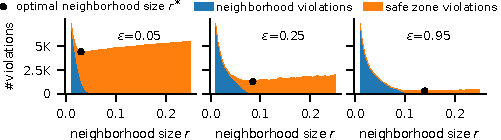
\includegraphics[width=1.0\columnwidth]{figures/impact_of_neighborhood_on_violations_three_error_bounds.pdf}}
	\caption{
	    The effect of neighborhood size $r$ on the number of violations while monitoring Rozenbrock function with four different approximation error bounds.
	}
	\label{fig:impact_of_neighborhood_on_violations_three_error_bounds}
\end{figure}


Figure~\ref{fig:impact_of_neighborhood_on_violations_three_error_bounds} shows the number of violations as a function of neighborhood size for four different approximation error bounds $\epsilon \in \{0.05, 0.25, 0.95\}$.
For a specific $\epsilon$, we observe the tradeoff
between neighborhood violations and safe zone violations.
Additionally, we see that permissive approximation error bounds (larger $\epsilon$) imply larger safe zones, resulting in fewer safe zone violations.
Increasing $\epsilon$ results in slightly more neighborhood violations, which we discuss below.
Lastly, we observe that neighborhood violations decrease when the neighborhood size increases, as expected.



Safe zone and neighborhood violation can hide each other.
Since the nodes check for neighborhood violation before checking the ADCD local constraint, some of the safe zone violations are concealed by neighborhood violations.
However, the opposite also happens.
When $\epsilon$ is small, the resulting small safe zone leads to many safe zone violations. 
When these are resolved, the coordinator updates $x_0$ and the neighborhood $\FB$, meaning that a future neighborhood violations are less likely. 
Therefore smaller $\epsilon$ results in fewer neighborhood violations.

\begin{algorithm}[t]
	\caption{Neighborhood Size Tuning}
	\begin{algorithmic}
		%
		\State $b \gets 1$
		\State \textbf{while} NoNeighborhoodViol(monitor with $r=b$) \textbf{do} $b \gets b / 2$
		\State $lo \gets b$, $hi \gets b$
		\State \textbf{while} AnySafezoneViol(monitor with $r=lo$) \textbf{do} $lo \gets lo / 2$
		\State \textbf{while} AnyNeighborhoodViol(monitor with $r=hi$) \textbf{do} $hi \gets 2\cdot hi$
		\State $R \gets 10$ equally spaced $r$ values in the range $[lo, hi]$
		\Return $\operatorname{argmin}_{r' \in R}$ NumTotalViolations(monitor with $r=r'$)
	\end{algorithmic}
	\label{algo:sub_domain_tuning}
\end{algorithm}



\betterparagraph{Tuning Procedure}
The optimal neighborhood size $r^*$, shown in Figure~\ref{fig:impact_of_neighborhood_on_violations_three_error_bounds} as a dot, is the neighborhood size that obtains the smallest number of violations in total.
The optimal size $r^*$ depends on the function, the data, and the allowed approximation error $\epsilon$.

To avoid the user needing to specify the neighborhood size $r$, AutoMon automatically tunes for the approximated optimal size $\hat{r}$.
This is done by running AutoMon on a small subset of the initial data and counting violations.
Algorithm~\ref{algo:sub_domain_tuning} is the tuning algorithm to find the approximated optimal neighborhood size $\hat{r}$.
It finds a low neighborhood size $r$ for which there are no safe zone violation and a high $r$ with no neighborhood violations, and then returns a neighborhood size in between with fewest total violations.
We evaluate the effectiveness of this tuning procedure in \S\ref{sec:eval-sub-domain-size}.

Since tuning is done on a small subset of the data, later changes in data distribution can mean $\hat{r}$ found by the tuning process becomes too small, causing unnecessary neighborhood violations.
In our experience this is rare, mostly when the error bound is very large.
We mitigate this using a simple heuristic:
whenever the coordinator observes $5 n$ consecutive neighborhood violations with no intervening safe zone violations, it multiplies $\hat{r}$ by 2.
We leave adaptive tuning of $r$ to future work.
